\appendix
\chapter{Modelle}
%Aufteilen in einzelne Modelle
\section{Raummodell}
\label{att:raummod}
\lstinputlisting[language=Modelica]{listings/room_model_listing.mo}


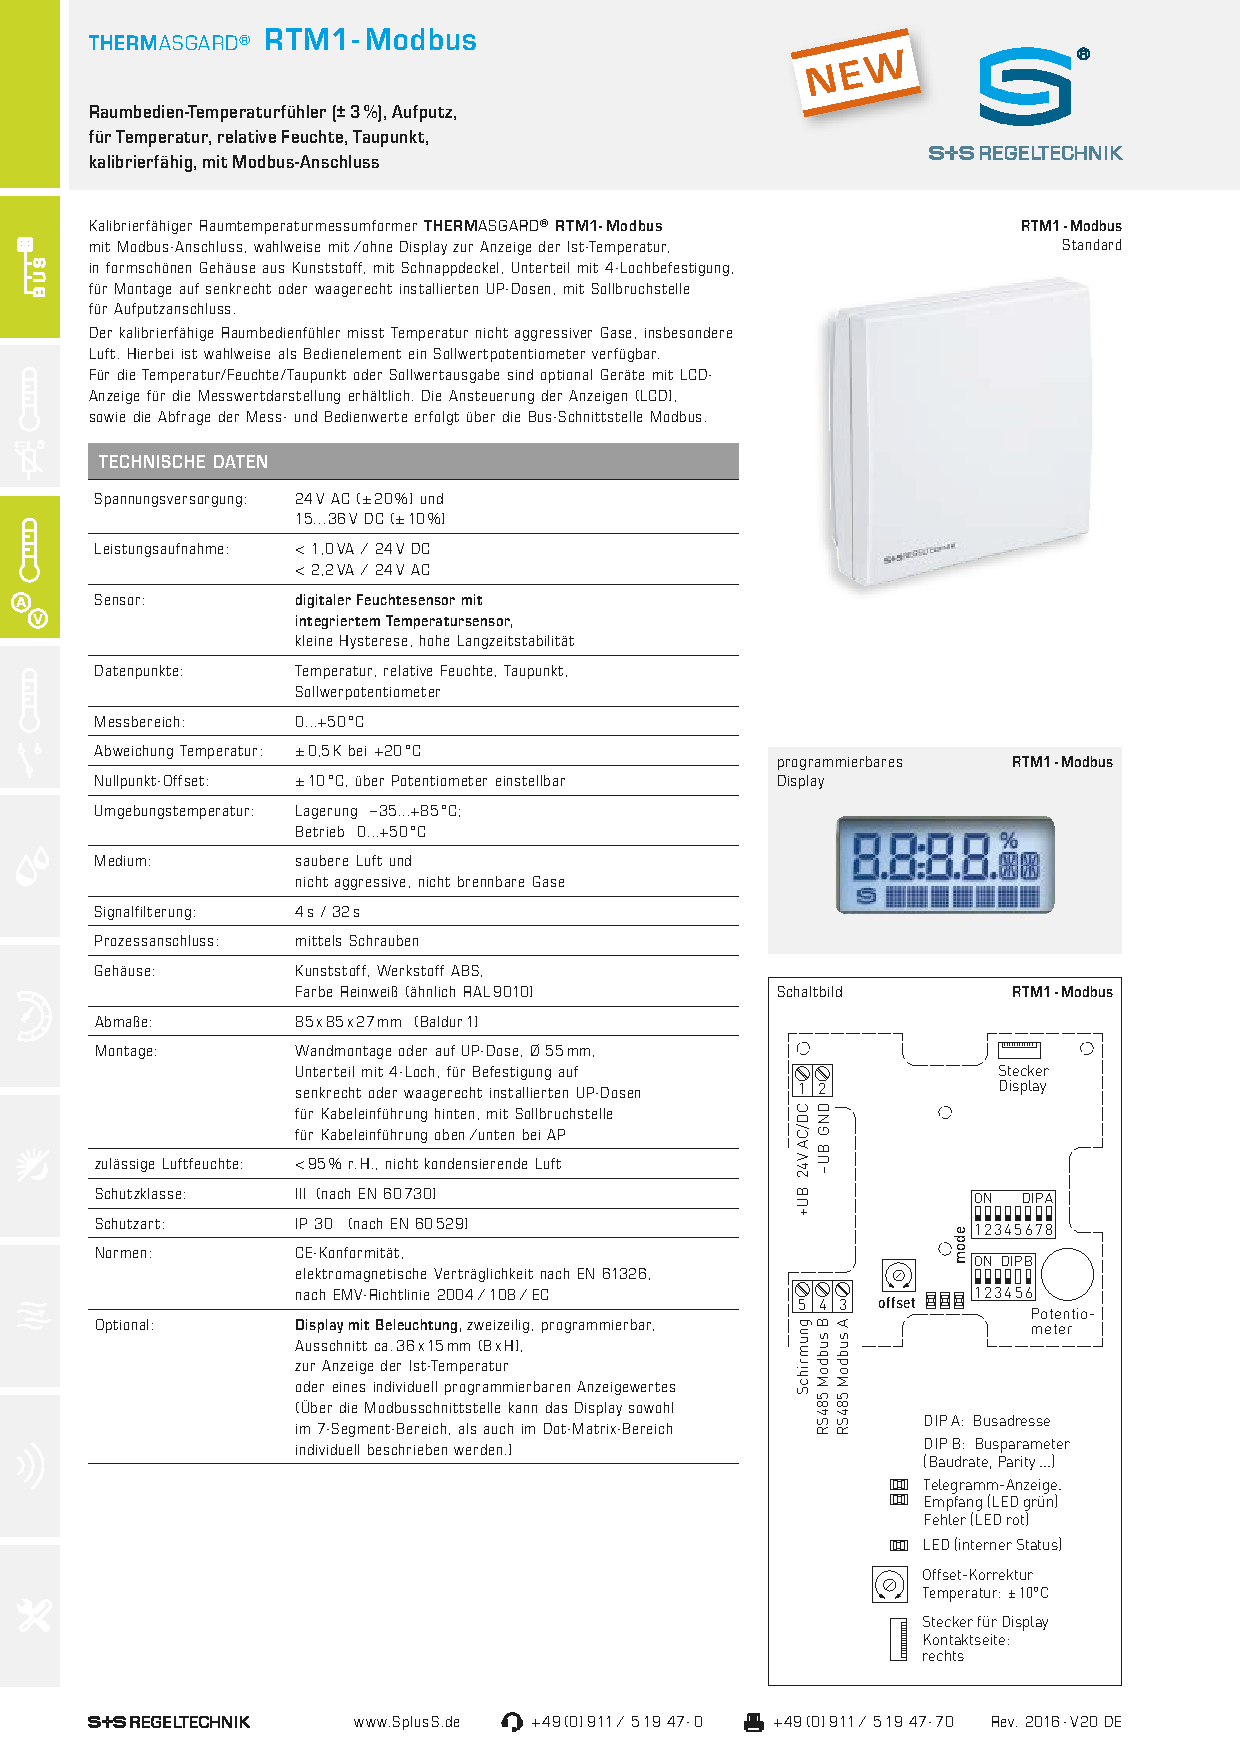
\includepdf[pagecommand={\chapter{Datenblätter}\section{THERMASGARD RTM1-Modbus Raumtemperaturfühler von S+S Regeltechnik}\label{att:rtm1}}, pages={1}, scale=0.7, offset=0.1cm -3cm]{anhang/rtm1}
\includepdf[pages={2}, scale=0.8]{anhang/rtm1}

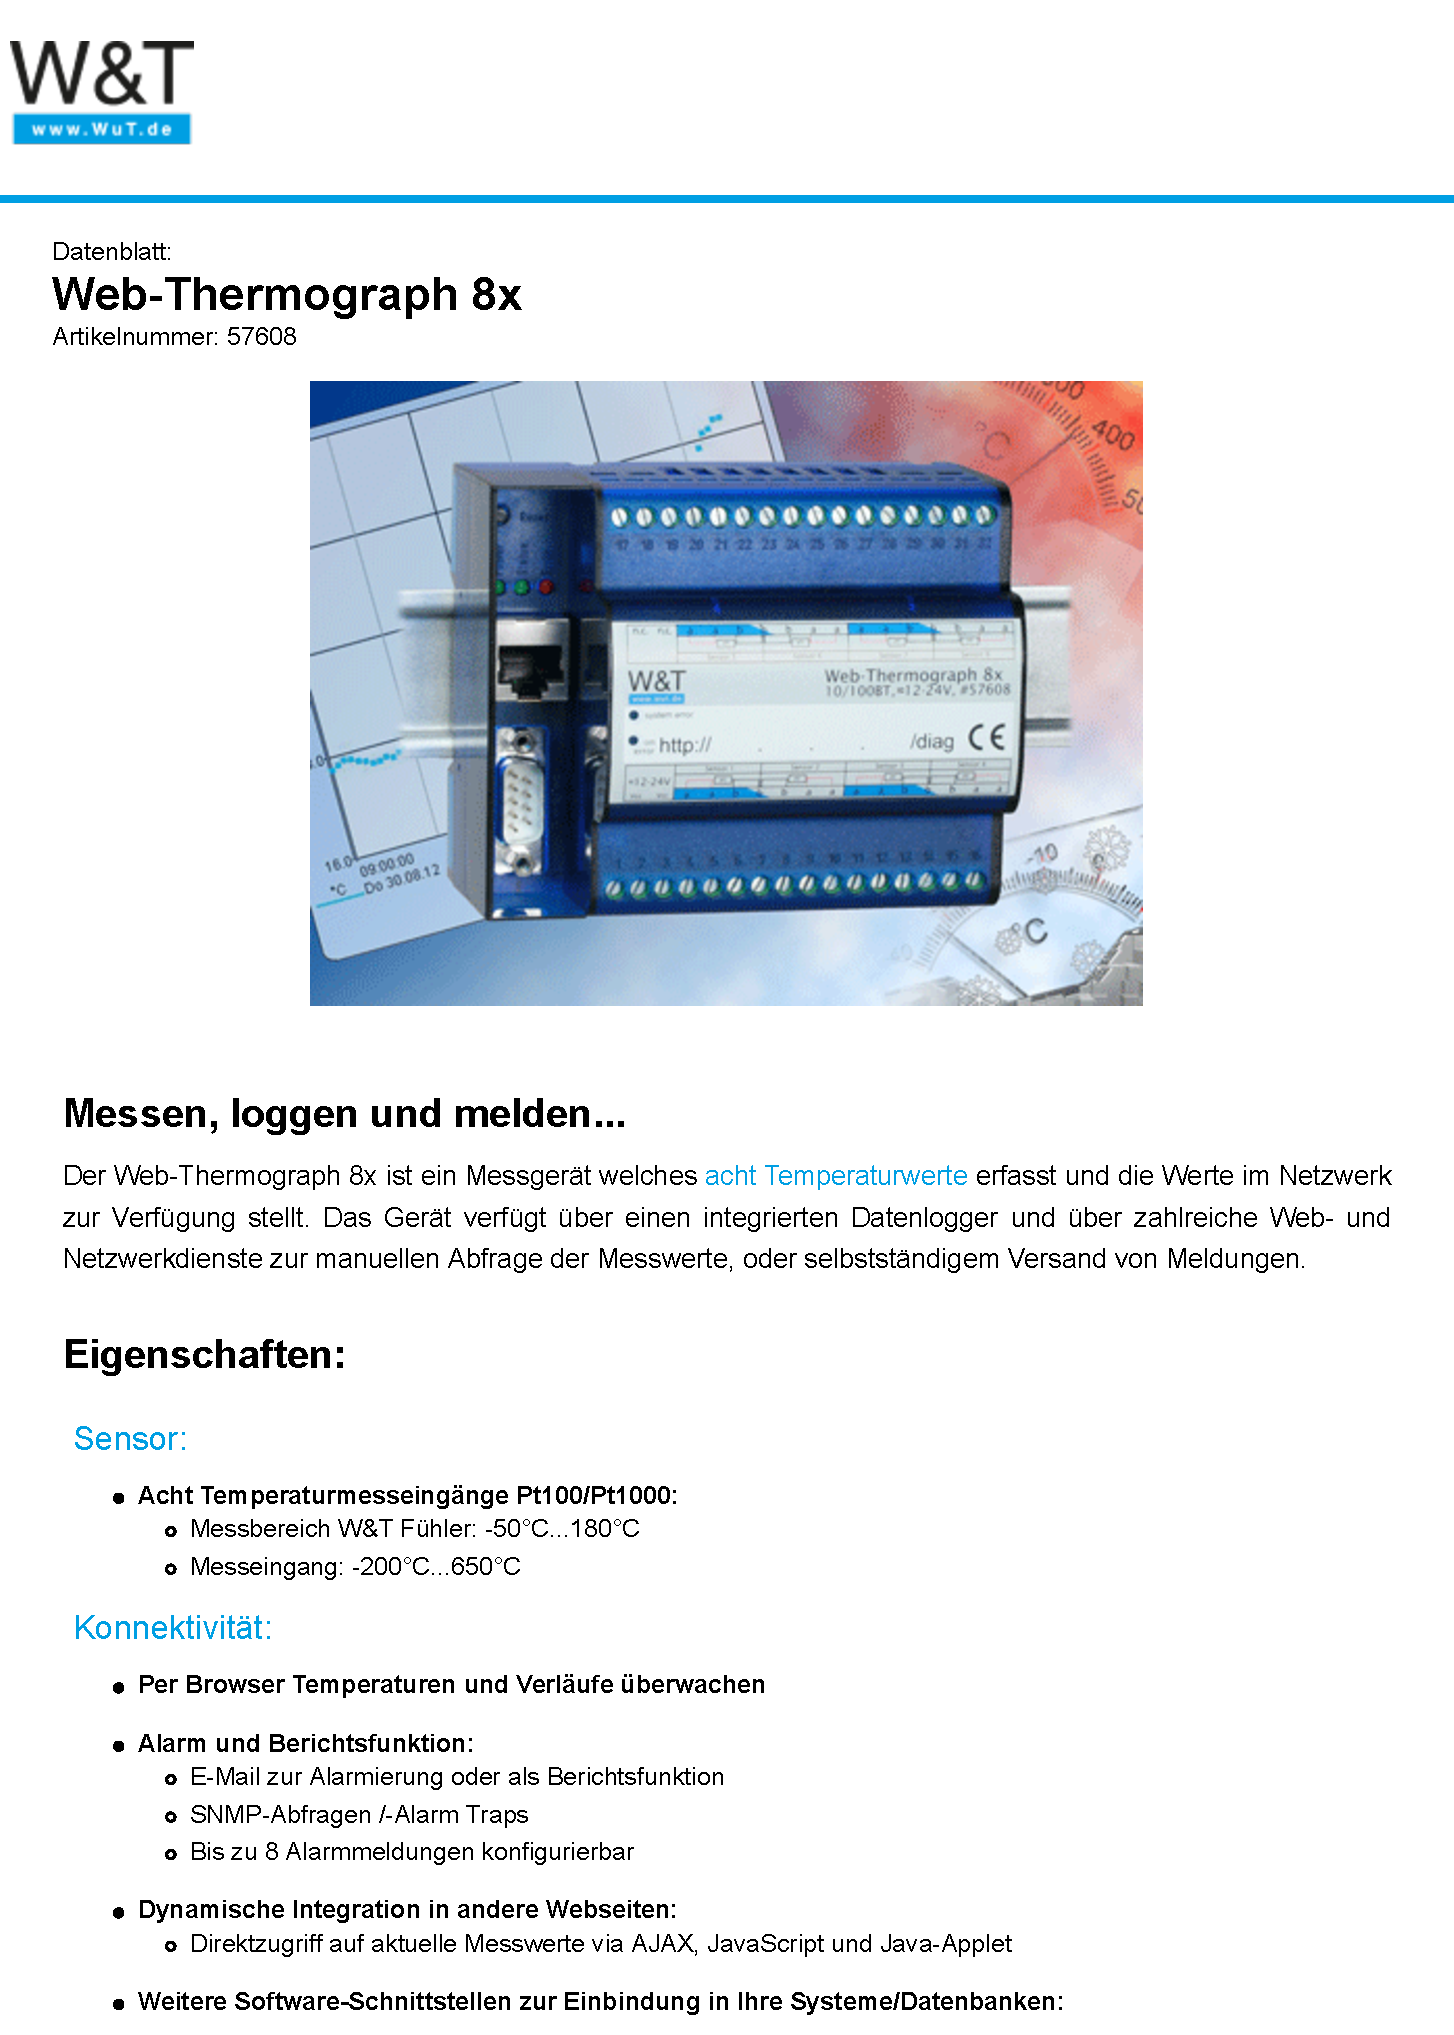
\includepdf[pagecommand={\section{Webthermograph 8x von WuT}\label{att:webtherm}}, pages={1}, scale=0.8, offset=0.1cm -2cm]{anhang/webthermograph8x}

\includepdf[pages={2-4}, scale=0.8]{anhang/multical}


\includepdf[pagecommand={\section{MULTICAL 602 Wärmemengenzähler von Kamstrup}\label{att:multi}}, pages={1}, scale=0.7, offset=0.1cm -2cm]{anhang/multical}

\includepdf[pages={2}, scale=0.8]{anhang/multical}



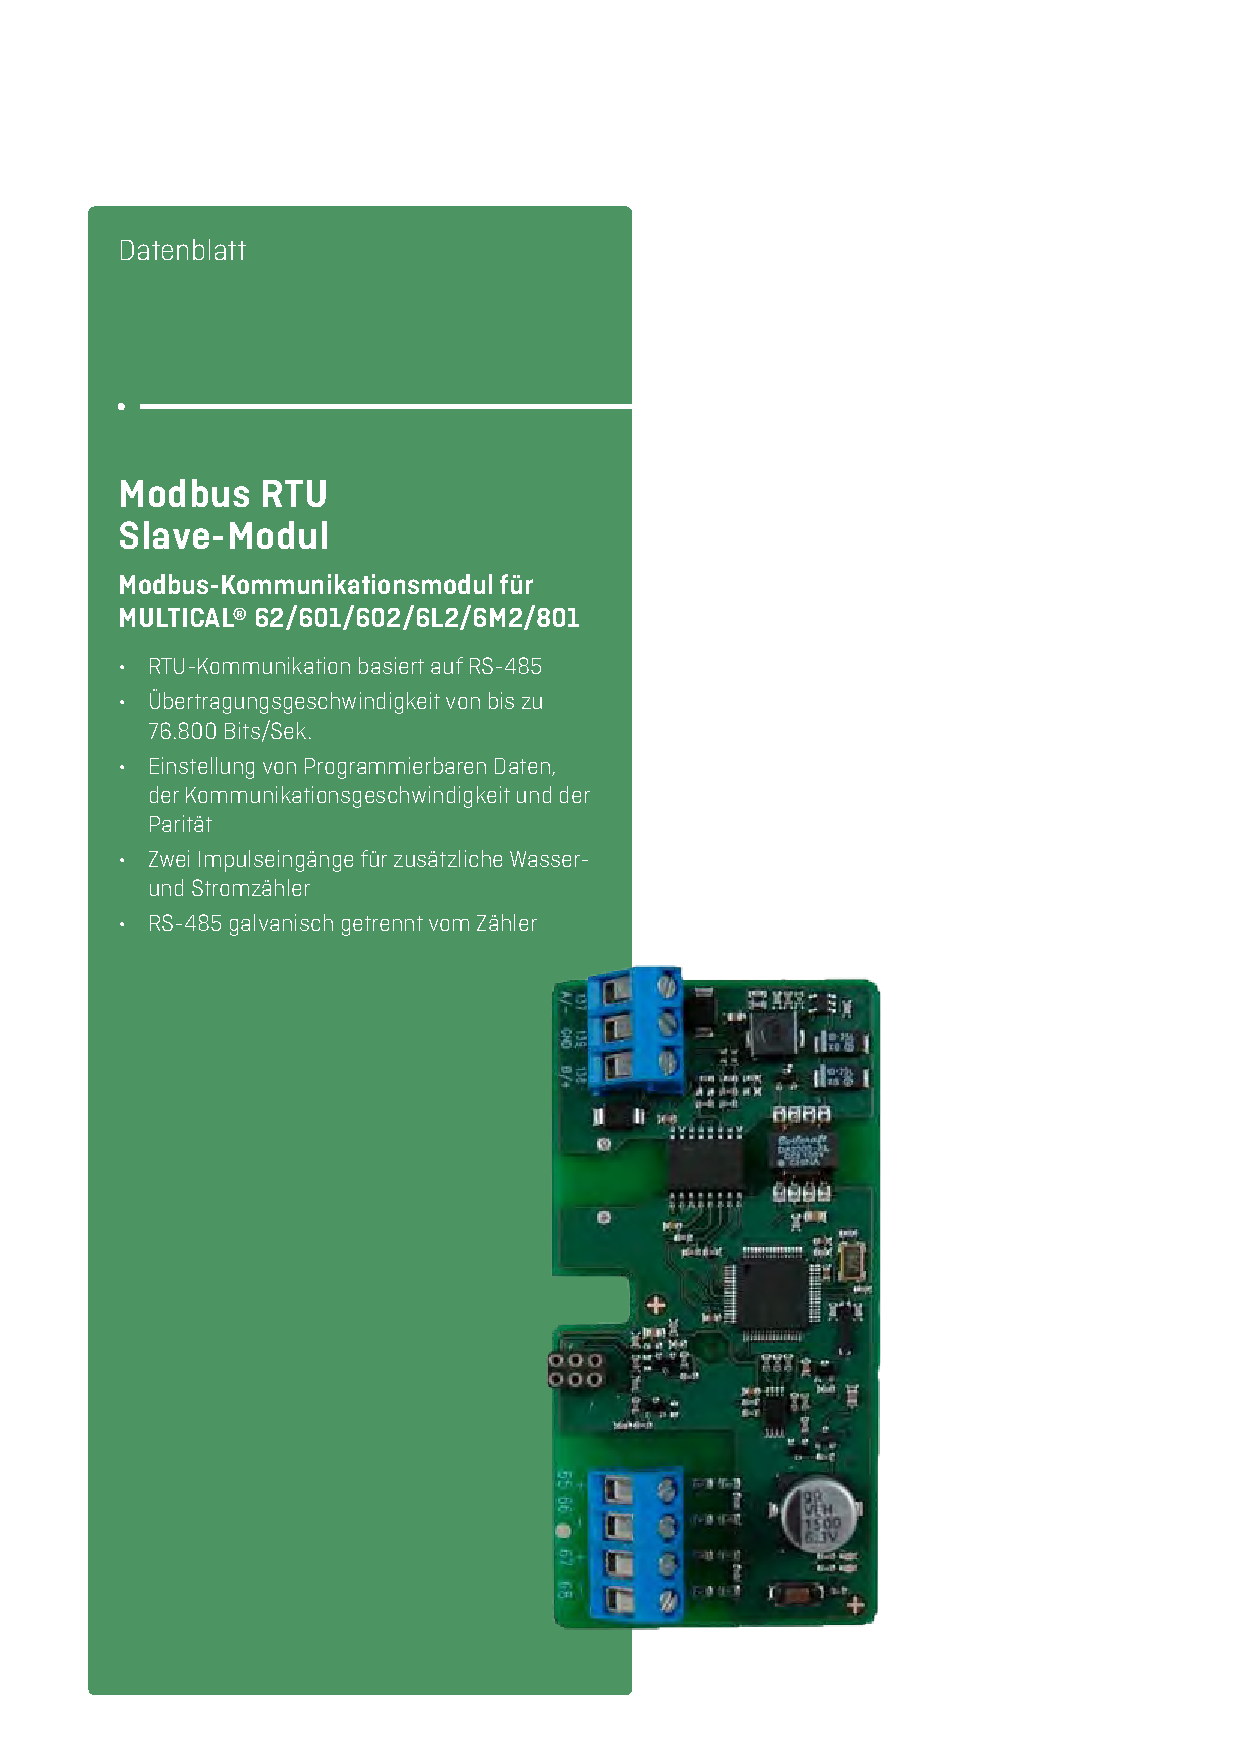
\includepdf[pagecommand={\chapter{Modbusadressmapping}\section{MULTICAL 602 Wärmemengenzähler von Kamstrup}\label{att:modbusmulti}}, pages={1}, scale=0.7, offset=0.1cm -2cm]{anhang/multicalmodbus}
\includepdf[pages={2-7}, scale=0.8]{anhang/multicalmodbus}


\includepdf[pagecommand={\section{THERMASGARD RTM1-Modbus Raumtemperaturfühler von S+S Regeltechnik}\label{att:rtm1modbus}}, pages={4}, scale=0.8, offset=0.1cm -2cm]{anhang/rtmmodbus}

\includepdf[pages={7-8}, scale=0.8]{anhang/rtmmodbus}

%\includepdf[pagecommand={\chapter{Datenblätter zum Rückkühlturm}\label{att:daten}\section{Datenblätter SorTech AG zum Rückkühlturm}}, pages={10}, scale=0.7, frame=true, offset=0.1cm -3cm]{attachement/Betriebsanleitung_AdK}
%\includepdf[pages={11-14}, scale=0.8, frame=true]{attachement/Betriebsanleitung_AdK}
%\includepdf[pagecommand={\section{Datenblatt der Wilo-Star Pumpe ST 20/9}\label{att:wilo}}, pages={1}, scale=0.8, frame=true]{attachement/wilo-star-st.pdf}
%\includepdf[pages={4}, scale=0.8, frame=true]{attachement/wilo-star-st.pdf}